\section{Metodología}

En esta sección se describe como fue el desarrollo del sistema, las herramientas usadas, así como detalles de la implementación. \\

Se desarrolló el sistema usando la metodología iterativa incremental. Esta metodología permite el desarrollo de un sistema incrementando sus capacidades cada iteración. En cada iteración se analiza, desarrolla y prueba un objetivo diferente, si al final de las pruebas el objetivo se cumplió se guarda el proyecto desarrollado y se empieza a trabajar con el siguiente objetivo, si el proyecto no pasa las pruebas se desecha y se vuelve a analizar.\\

En la figura \ref{fig:arquitectura} se muestra el diagrama a bloques del sistema a desarrollar, el primer bloque es la captación de los datos de un objeto, el segundo el clasificador que hace uso del AGC para obtener la representación del objeto.\\

    \begin{figure}[!htb] 
        \centering
        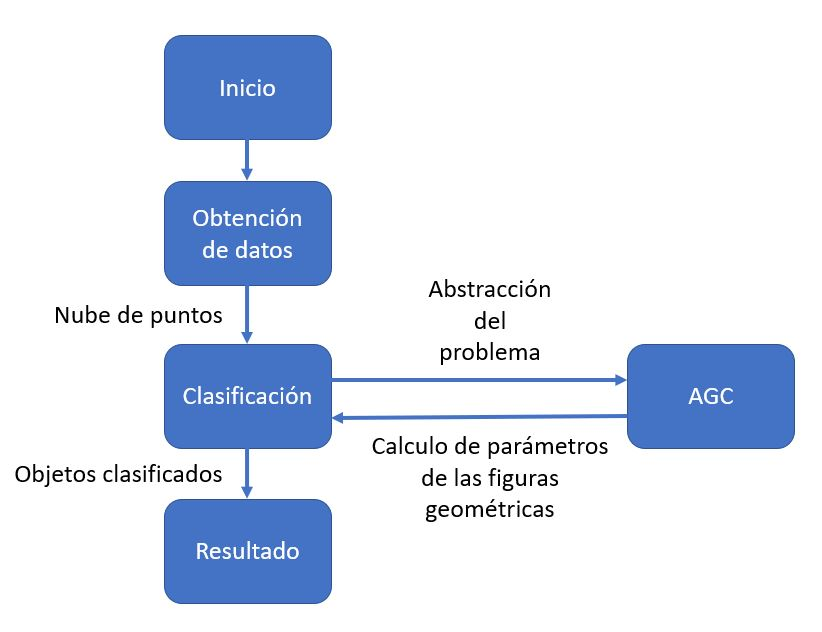
\includegraphics[width=0.7\textwidth]{01Introduccion/imagenes/arquitectura_del_sistema.JPG}
        \caption{Diagrama a bloques del sistema}
        \label{fig:arquitectura}
    \end{figure}


Como primer objetivo se planteó la obtención de datos del Kinect, luego la clasificación de los objetos y por último la integración del AGC.\\
